In this section, we will focus on the analysis of different databases based on the  evaluation of XMark queries. BaseX, MongoDB, Couchbase and RethinkDB are completely different database systems with their own data models and different query languages.  Due to their completely different nature, a query of a database would perform better than others if data was normalized according to their specified data model. For example, BaseX would probably perform better if the data was normalized. Therefore, our goal is not to compare queries between these databases, but to evaluate the results individually.  All databases have been tested with 6 different size XMark dataset as mentioned in ~\ref{benchmark-database-size}. Firstly, the results  of the four systems will be analyzed individually. Secondly, the performance of all the databases of the 111MB dataset will be examined together.

\subsection{MongoDB}
Figure~\ref{fig:xmark-result-mongodb-all} presents the time measurements of XMark queries in MongoDB. MongoDB automatically uses all the free memory of a machine for its cache. The result of the queries will be explained below:
\begin{itemize}
\item The simplest query Q1 was the most efficient query. It was executed in less than 4ms for all database instances, because the MongoDB representation of the query boils down to a simple \textit{\_id} selection.
\item Q2 and Q3 were relatively slow queries due to the number of stages in the aggregation pipeline. Even though two secondary indexes were used, the performance of these queries was not competitive to other systems. 
\item The \textit{count} operation in MongoDB is faster than in other NoSQL databases. Q5 and Q6 are used to count the number of documents in a collection. Q5 contains a comparison operator, and the secondary index in field \textit{price} helped to accelerate the execution. Figure~\ref{fig:xmark-mongodb-index-noindex} illustrates the efficiency of the two queries Q5 and Q13, in which the execution time improved exponentially after the application of the secondary indexes. Q6 is even simpler, as it only contains a \textit{count()} function, and thus hardly consumes any time.

\item Among the join queries, Q8 and Q9 yielded the best results. Once again, the indexes created in these two queries improved the performance. 
But in case of Q10, the complex result generation could not be completed in the given time frame for the two largest database instances. This was probably due to the large result, which does not simply contain database results, but is newly generated by the query. The value join queries in Q11 and Q12 have to deal with many read operations, due to the manual looping with the \textit{forEach} expression.

\item The secondary index in Q13 helped to keep execution time low. As mentioned earlier, Fig.~\ref{fig:xmark-result-mongodb-13} shows the elapsed time with and without index. Q14 is used to search for sub-strings. Execution time scales linearly.

\item Compared to the XQuery representation, queries Q15 and Q16 are relatively complex in all NoSQL databases including MongoDB, because the child axes of the original query need to be rewritten to various aggregation stages. The results produced by these queries were not exactly the same as for XQuery but the performance was in the same order of magnitude. The performance of Q17 was similar to other systems.

\item  The user-defined function can be implemented only from mapreduce. The \ref{mongodb-q-18}, utilized a lot of resources for the two largest database instances. The mapreduce that uses the manual function call from other document made query inefficient. 

\item In Q19, a new field \textit{item} is generated. Because of that, the performance decreases, because  MongoDB has to use an aggregation pipeline for the new field. The Query would be much faster if the result were returned without a new field by using the \textit{find()} function.

\item Finally, cardinalities are grouped and returned in Q20. The mapreduce is implemented for this query. As mentioned in Section~\ref{mongo-query-model}, advanced queries can be achieved in two ways. Q20 is tested in both aggregation pipeline and mapreduce. In pipeline, the query is complex and has to perform in many stages. Mapreduce is flexible, easy to implement and scalable. MongoDB breaks the query in multiple parts and process accross the nodes. But in a standalone mode, query is relatively slow. Figure ~\ref{fig:xmark-result-mongodb-pipeline-mapreduce} shows the result of Q20 in both mapreduce and pipeline. The Mapreduce is single-threaded, therefore it is relatively slower to aggregation pipeline.
\end{itemize}
\begin{figure}[hbt]
	\centering
	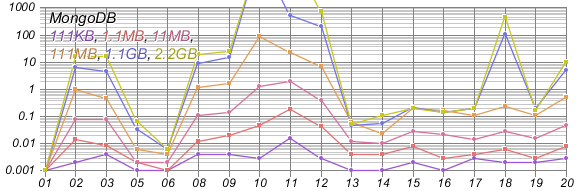
\includegraphics[width=0.95\textwidth]{img/result/mongodb/mongodb-all-18-20}
	\caption{XMark queries in MongoDB}
	\label{fig:xmark-result-mongodb-all}
	
\end{figure}	
\begin{figure}[hbtp]
	\centering
	\subfloat[Q5]{
		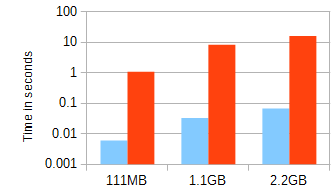
\includegraphics[width=0.45\textwidth]{img/result/mongodb/mongodb-q5-index-noindex}
		\label{fig:xmark-result-mongodb-5}
	}
	\centering
	\subfloat[Q13]{
		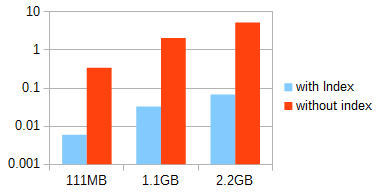
\includegraphics[width=0.45\textwidth]{img/result/mongodb/mongodb-q13-index-noindex}
		\label{fig:xmark-result-mongodb-13}
	}
	\caption{MongoDB queries with and without secondary index in different database instances}
	\label{fig:xmark-mongodb-index-noindex}
\end{figure}

\begin{figure}[hbtp]
	\centering
	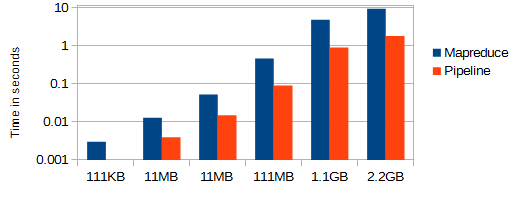
\includegraphics[width=0.95\textwidth]{img/result/mongodb/mongodb-mapreduce-pipeline}
	\caption{Aggregation pipeline and Mapreduce result of Q20 in MongoDB}
	\label{fig:xmark-result-mongodb-pipeline-mapreduce}
	
\end{figure}

\subsection{Basex}
The results of all six different databases in BaseX is shown in Figure~\ref{fig:xmark-result-basex-all}. All the queries were tested with text, attribute and full text indexes. 
\begin{itemize}
\item The query Q1 contains the predicates with an equality comparison and a single result was returned. This query was completed in less than 5ms in all database instances.  The path and attribute index of BaseX reduces the execution time.

\item Positional predicates are defined in Q2 and Q3, and the resulting items are returned into new elements. BaseX performed one of the best result among all systems. 

\item Queries Q5 and Q6 contain the \textit{count()} function and both were comparatively better than RethinkDB and Couchbase, but as it has been seen in the previous section, these queries were performed most efficiently by MongoDB.
\item 
Among the join queries, the database instances larger than 11MB were not completed in Q11 and Q12. They were also the most inefficient queries in BaseX.  For reference join queries Q8 and Q9, the attribute index is utilized. The time taken by these two queries is comparable to that of MongoDB. Q10 was not completed in given time frame for two largest instances but among the completed instances, the results were similar to those of all database systems 
\item The query Q13 was completed in all databse instances in less than a second. The performance is competitive in all systems but RethinkDB produces best the results. 
\item  The \textit{contains()} function in query Q14 is executed in numerous atomized text nodes. This query is in the NoSQL databases substring search of the stringified text of an object. NoSQL datbases were sligly faster than BaseX. 

\item In Q15-Q17, the results were competitive in all databases. The Q19 consumes most resources for sorting the data. This query is faster in MongoDB compared to BaseX.

\item Finally, BaseX  had produced linear result in all database instances for the aggregation query Q20. It is relatively faster than MongoDB, but Couchbase generated competitive results. 
\end{itemize}
\begin{figure}[hbt]
	\centering
	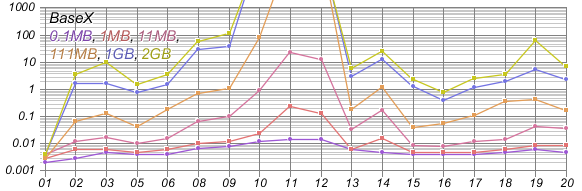
\includegraphics[width=0.95\textwidth]{img/result/basex/basex-all}
	\caption{XMark queries in BaseX}
	\label{fig:xmark-result-basex-all}
\end{figure}

\subsection{RethinkDB}
All the time evaluation of XMark queries in RethinkDB is given in Fig.~\ref{fig:xmark-result-rethinkdb-all}. 
\begin{itemize}
\item Query \ref{rethink-q-1} needed more time compared to MongoDB and BaseX in average. 
 \item  
  ReQL has way better features  to handle arrays and objects of JSON than other NoSQL databases. The chainable query was used as a pipeline, but unlike MongoDB's pipeline, RethinkDB runs a query on a server at once without intermediate result. The queries Q2 and Q3 far better than MongoDB and are competitive to other databases. 
 \item
 Queries Q5 and Q6 were comparatively slow in  RethinkDB. The \textit{count()} operation in RethinkDB is always slow due to its streaming property. It executes everything in the server, most of the stream operations including \textit{filter} run lazily. The \textit{run} function returns the results as soon as the first block of data is available. It does not load whole table data  at once but only after client iterate over the cursor. In case of \textit{count()}, the query has to wait until all the data is loaded.
 
 
 \item Since we have previously mentioned the support of join query in ~\ref{xmark-rethinkdb}, RethinkDB was not able to take advantages of native joins in Q8 and Q9. This is once again due to the \textit{count} function used in these queries. RethinkDB produces the best result inQ11 and Q12  among all systems. The join operation with secondary indexes accelerated the performances.
 
\item In query Q13,  a secondary index is utilized on \textit{regions} field of the table \textit{regions} that produces comparable result to MongoDB but better than BaseX.  

\item The query Q20 was once again slow in RethinkDB due to cardinalities at the end of the query. All the grouping and categorizing operations were a lot faster than the \textit{count()} at the end. 
\end{itemize}

\begin{figure}
	\centering
	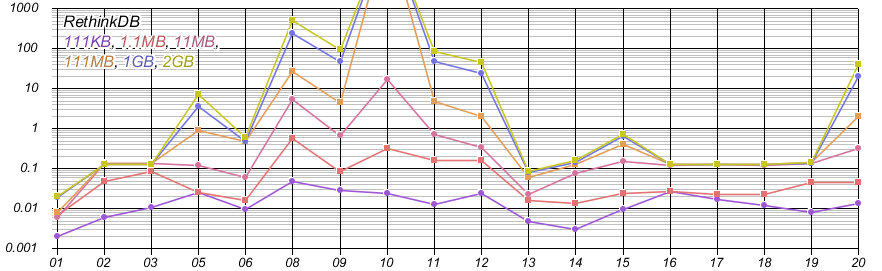
\includegraphics[width=0.95\textwidth]{img/result/rethinkdb/rethinkdb-all}
	\caption{XMark queries in RethinkDB}
	\label{fig:xmark-result-rethinkdb-all}
\end{figure}

\subsection{Couchbase}
Each Couchbase bucket is assigned RAM quota for caching data, therefore, the performance of a query depends on the amount of RAM allocated at the time of bucket creation. Couchbase was tested on five XMark instances and Figure~\ref{fig:xmark-result-cb-all} explains the query performance of individual queries\todo{put all database images}. The queries with pre-defined reduce functions like \textit{\_count} or \textit{\_sum} had produce very competitive results with other database systems.

The first query Q1 is bit slower than others in Couchbase as a result of SDK interface for query. Two queries Q2 and Q3 has similar result as that of RethinkDB  but Q5 and Q6 had produced comparatively better result due to its pre-defined reduce function \textit{\_count} in mapreduce. among the join queries, the 1.1 GB instance could not completed in Q9 and Q10 in defined time limit. For query Q9 the Node.js had to performed manuel join in three different views that lead longer time. 
The string search query in Q14 was the best queries in Couchbase. The reason was the easy object to string conversion and the index on the view. Another best result in Couchbase is aggregation query Q20, which is able to use pre-defined \textit{\_sum} in reduce part of Mapreduce. 

\begin{figure}
	\centering
	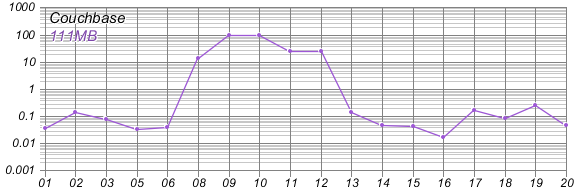
\includegraphics[width=0.95\textwidth]{img/result/cb/cb-all}
	\caption{XMark queries in Couchbase}
	\label{fig:xmark-result-cb-all}
\end{figure}

\subsection{Summary}
Even though our aim is not to compare query performance in different systems directly, it would be interesting to see how these queries look like beside one another. Figure~\ref{fig:xmark-result-1-all-new} illustrates all the queries for different database systems for the 111MB instance of XMark. MongoDB and BaseX had produced the best result in Q1. In Q2 and Q3, all database except MongoDB had an identical result, but in Q5 and Q6, MongoDB was the clear leader, followed by Couchbase and BaseX, whereas RethinkDB was lagging behind other databases. In the join queries, the results produced by different databases were mixed in nature. MongoDB and BaseX were fastest for Q8 and Q9, followed by Couchbase and RethinkDB. In Query Q10, RethinkDB has failed to return a result in a given time frame, but all other databases displayed similar results. The value join queries Q11 and Q12 were the best queries for RethinkDB, followed by MongoDB and Couchbase; but BaseX could not complete the query. Even though Q13 has similar results for all systems, RethinkDB had generated the best performance (followed by MongoDB) due to the application of efficient index structures. The full text search query Q14 is a substring search. This allows the query to be executed faster. The complex XPath queries Q15 and Q16 of Basex has produced better results in Couchbase compared to RethinkDB and MongoDB. This is similar for Q17-Q19, but in Q20, Couchbase was the leader, followed by BaseX, MongoDB, and RethinkDB. 

It can be observed that the NoSQL queries that were able to benefit from secondary indexes performed better than BaseX with some exceptions. Even though some NoSQL databases do not support join queries, the results they produced were competitive in nature. The reason for this is that the data was normalized for NoSQL databases, whereas BaseX was operating on the original data and queries. BaseX would clearly have performed better if the queries or XML data had been normalized as well.
% NoSQL database has efficient read operation 
\begin{table}[H]
\tiny
\begin{tabular}{|c|c|c|c|c|c|c|c|c|c|c| c|c|c|c|c|c|c|c|c|c|c|  } 
   db &  1 & 2 & 3 & 5 & 6  & 8 & 9 & 10  & 11 & 12 & 13 & 14 & 15 & 16 & 17 & 18 & 19 & 20 \\
 \hline
M\hbox{\pdfliteral{1 1 0 rg}\vrule height2mm width2mm depth0mm\pdfliteral{0 g}} & .00 & .75 & .78 & .01 & .00 & 1.17 & 1.65 & 87.25 & 23.13 & 7.21 & .05 & .55 & .20 & .17 & .11 & .22 & .11 & .21 \\
B\hbox{\pdfliteral{0 0 1 rg}\vrule height2mm width2mm depth0mm\pdfliteral{0 g}} & .04 & .19 & .17 & .10 & .19 & 2.31 & 2.43 & 89.36 & udf & udf & .36 & 1.23 & .08 & .08 & .15 & .36 & .52 & .19 \\
C\hbox{\pdfliteral{1 0 0 rg}\vrule height2mm width2mm depth0mm\pdfliteral{0 g}} & .04 & .14 & .08 & .03 & .04 & 13.2 & 98.1 & 94.1 & 24.1 & 26.1 & .13 & .05 & .04 & .02 & .17 & .09 & .27 & .05 \\
R\hbox{\pdfliteral{0 1 0 rg}\vrule height2mm width2mm depth0mm\pdfliteral{0 g}} & .01 & .14 & .14 & .94 & .68 & 26.76 & 4.53 & .00 & 4.80 & 2.10 & .02 & .18 & udf & .13 & .13 & .13 & .14 & 2.04 \\
\end{tabular}
\end{table}
\begin{figure}[H]
	\centering
	\subfloat[XMark queries of 111MB data in all DBMS]{
		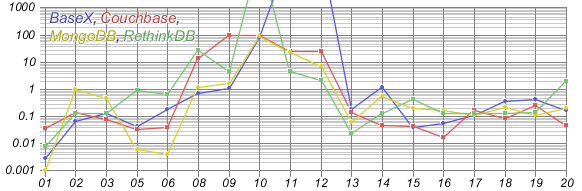
\includegraphics[width=0.85\textwidth]{img/result/1/1-all-new}		\label{fig:xmark-result-1-all-new}
	}
	\caption{XMark queries of 111MB data in all DBMS}
	\label{fig-xmark-result-1-all-queries}
\end{figure}